\thispagestyle{plain}
\section{Results}
\indent

Both implemented models in Mars solver \cite{mars} were tested for the accuracy of the results with real data. 

\subsection{Testing of Drucker-Prager model}
\indent
 
For testing accuracy of implemented Drucker-Prager model we choose experimental test taken from \cite{Deuch_phd_thesis}, where we can find compression test of the polymer mortar. As you can see in the Fig. \ref{obr:test_param}, it is a classic compression test, when is examined element compressed with testing equipment. Specific parameters of the tested element and equipment you can find in the Fig. \ref{obr:test_param}. As you can se in the Fig. \ref{obr:Compresion_test}, apparature is in the modeled object simplified to the two plates that are perpendicular to each other. In the model is the test specimen completely fixed to the bottom plate, but the top plate affect the sample with a friction force, so it can move on the plate, and also the plate can rotate.


\begin{figure}[h!]
	\centering
	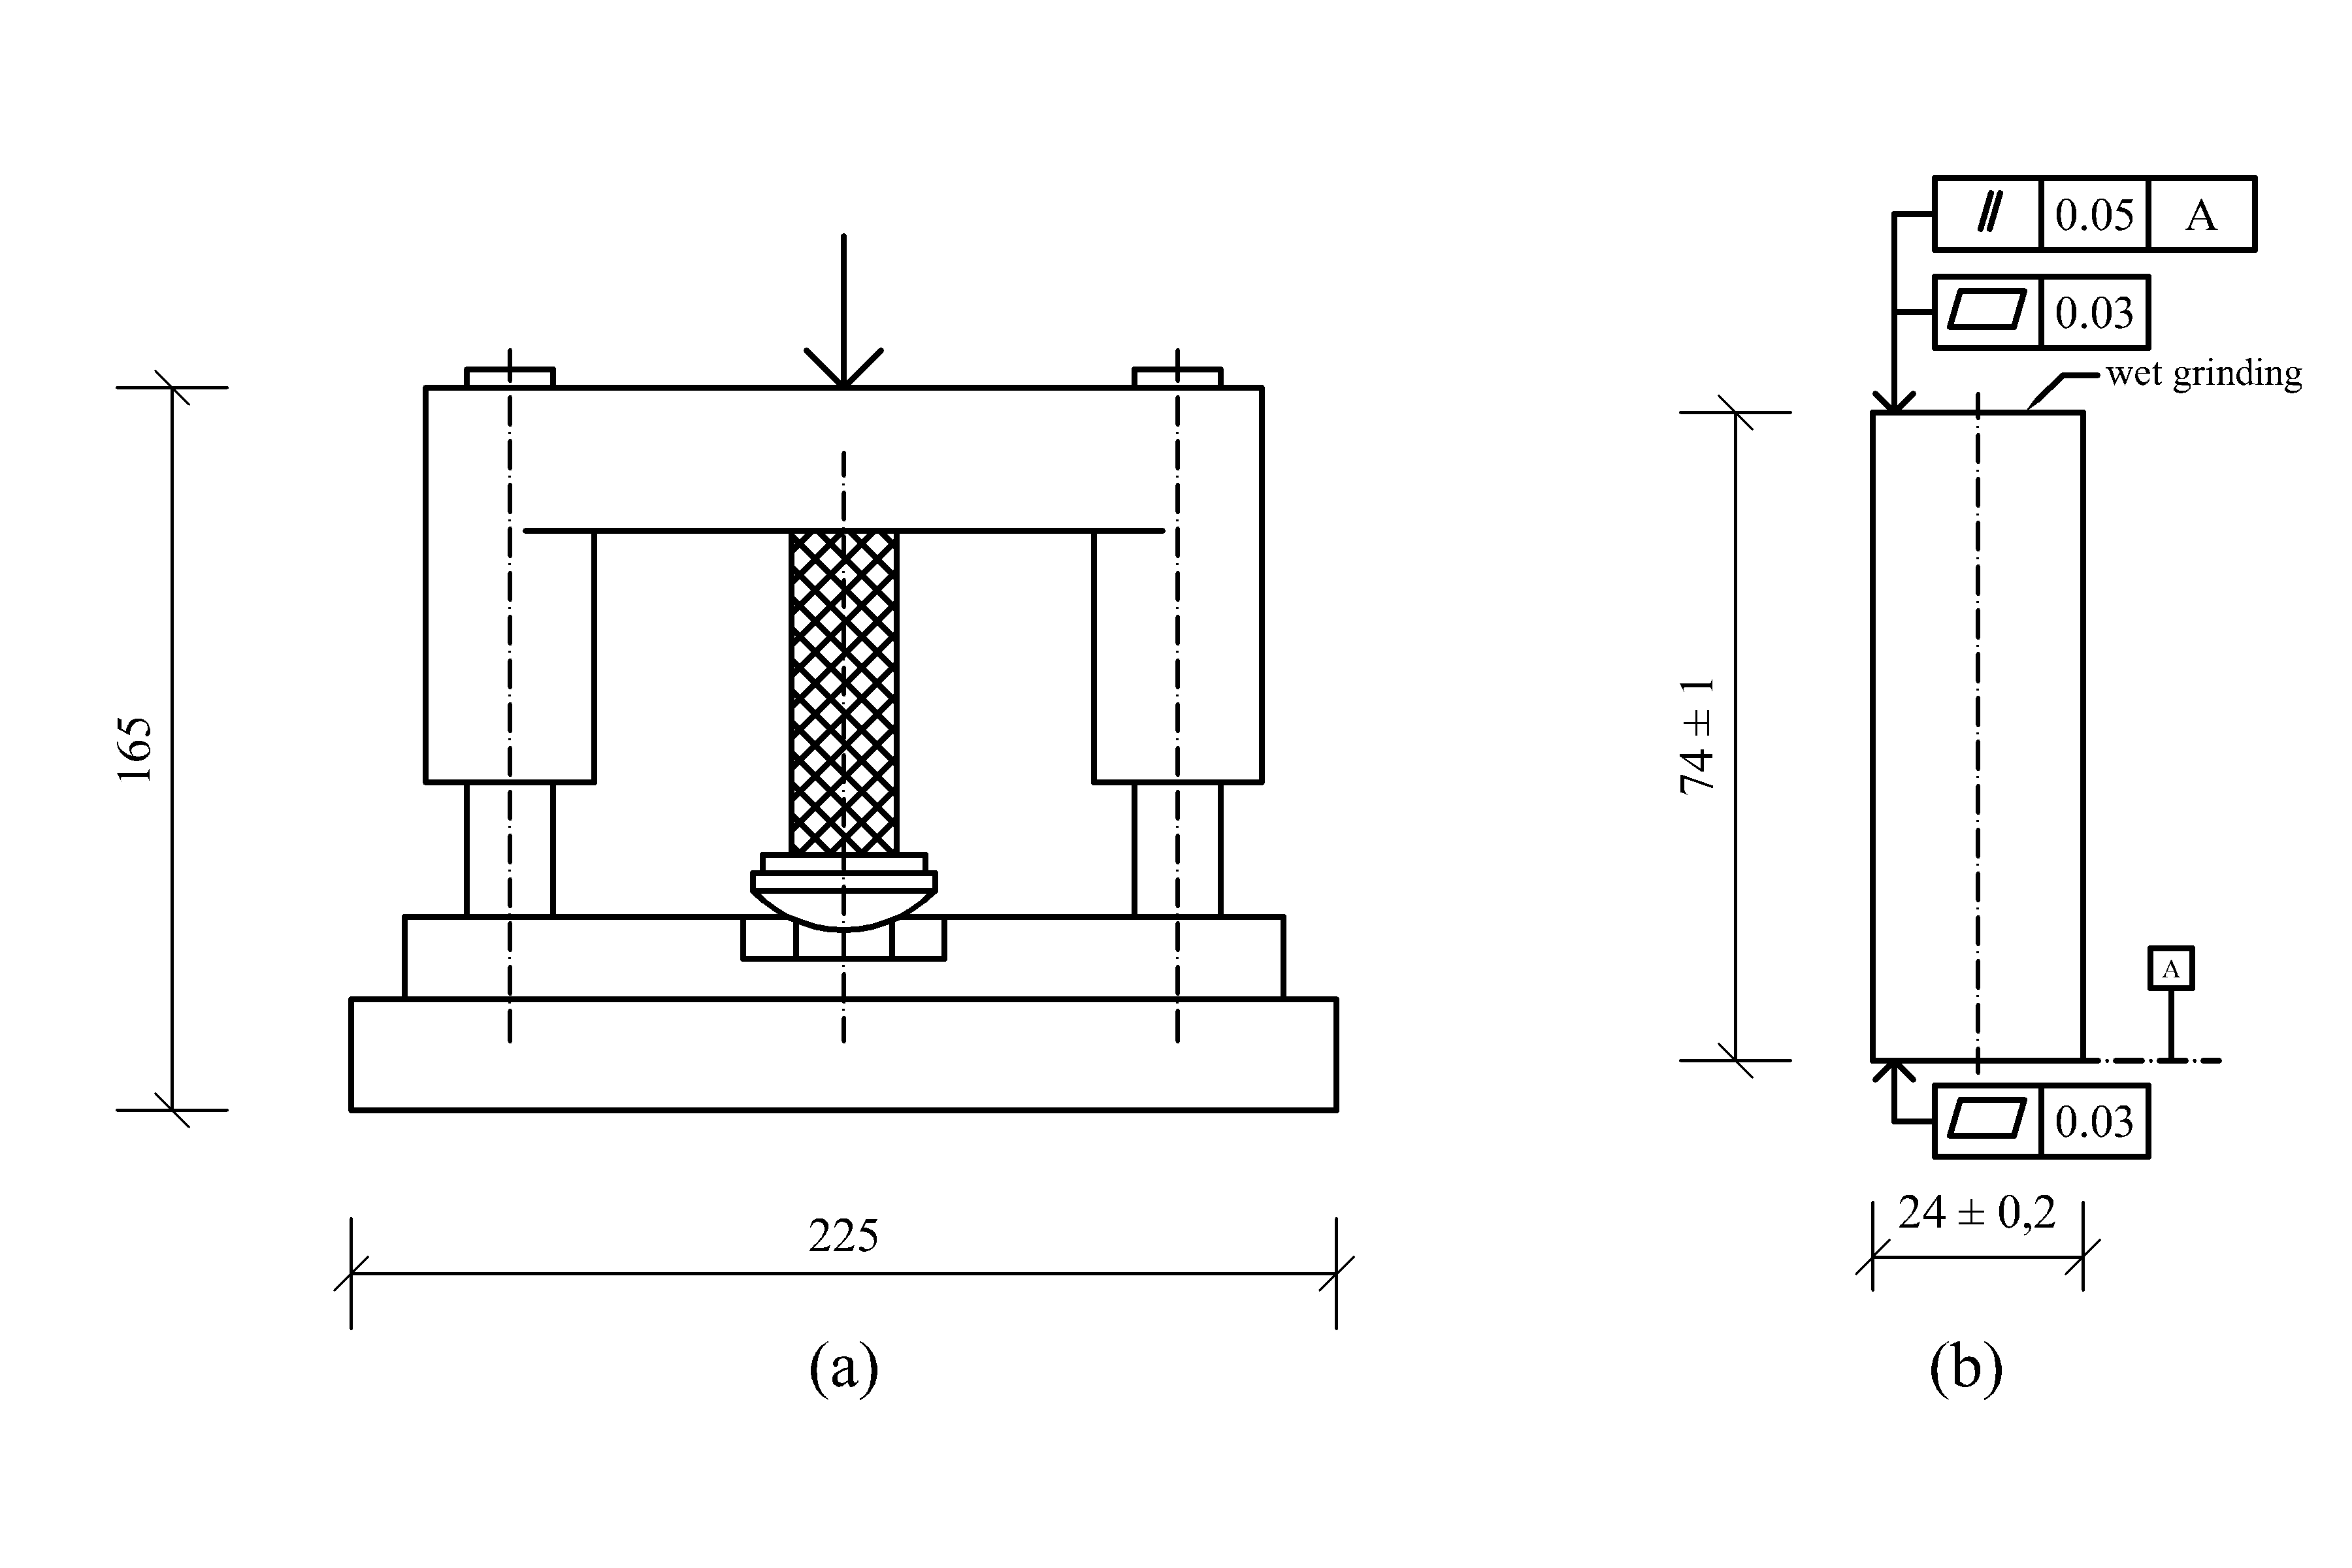
\includegraphics[width=0.8\textwidth]{obrazky/test_parameters.png}
	\caption[Compression test parameters]{Compression test parameters \cite{Deuch_phd_thesis}: a) dimensions of the apparature; b) parameters of the specimen.}\label{obr:test_param}
\end{figure}

\begin{figure}[h!]
	\centering
	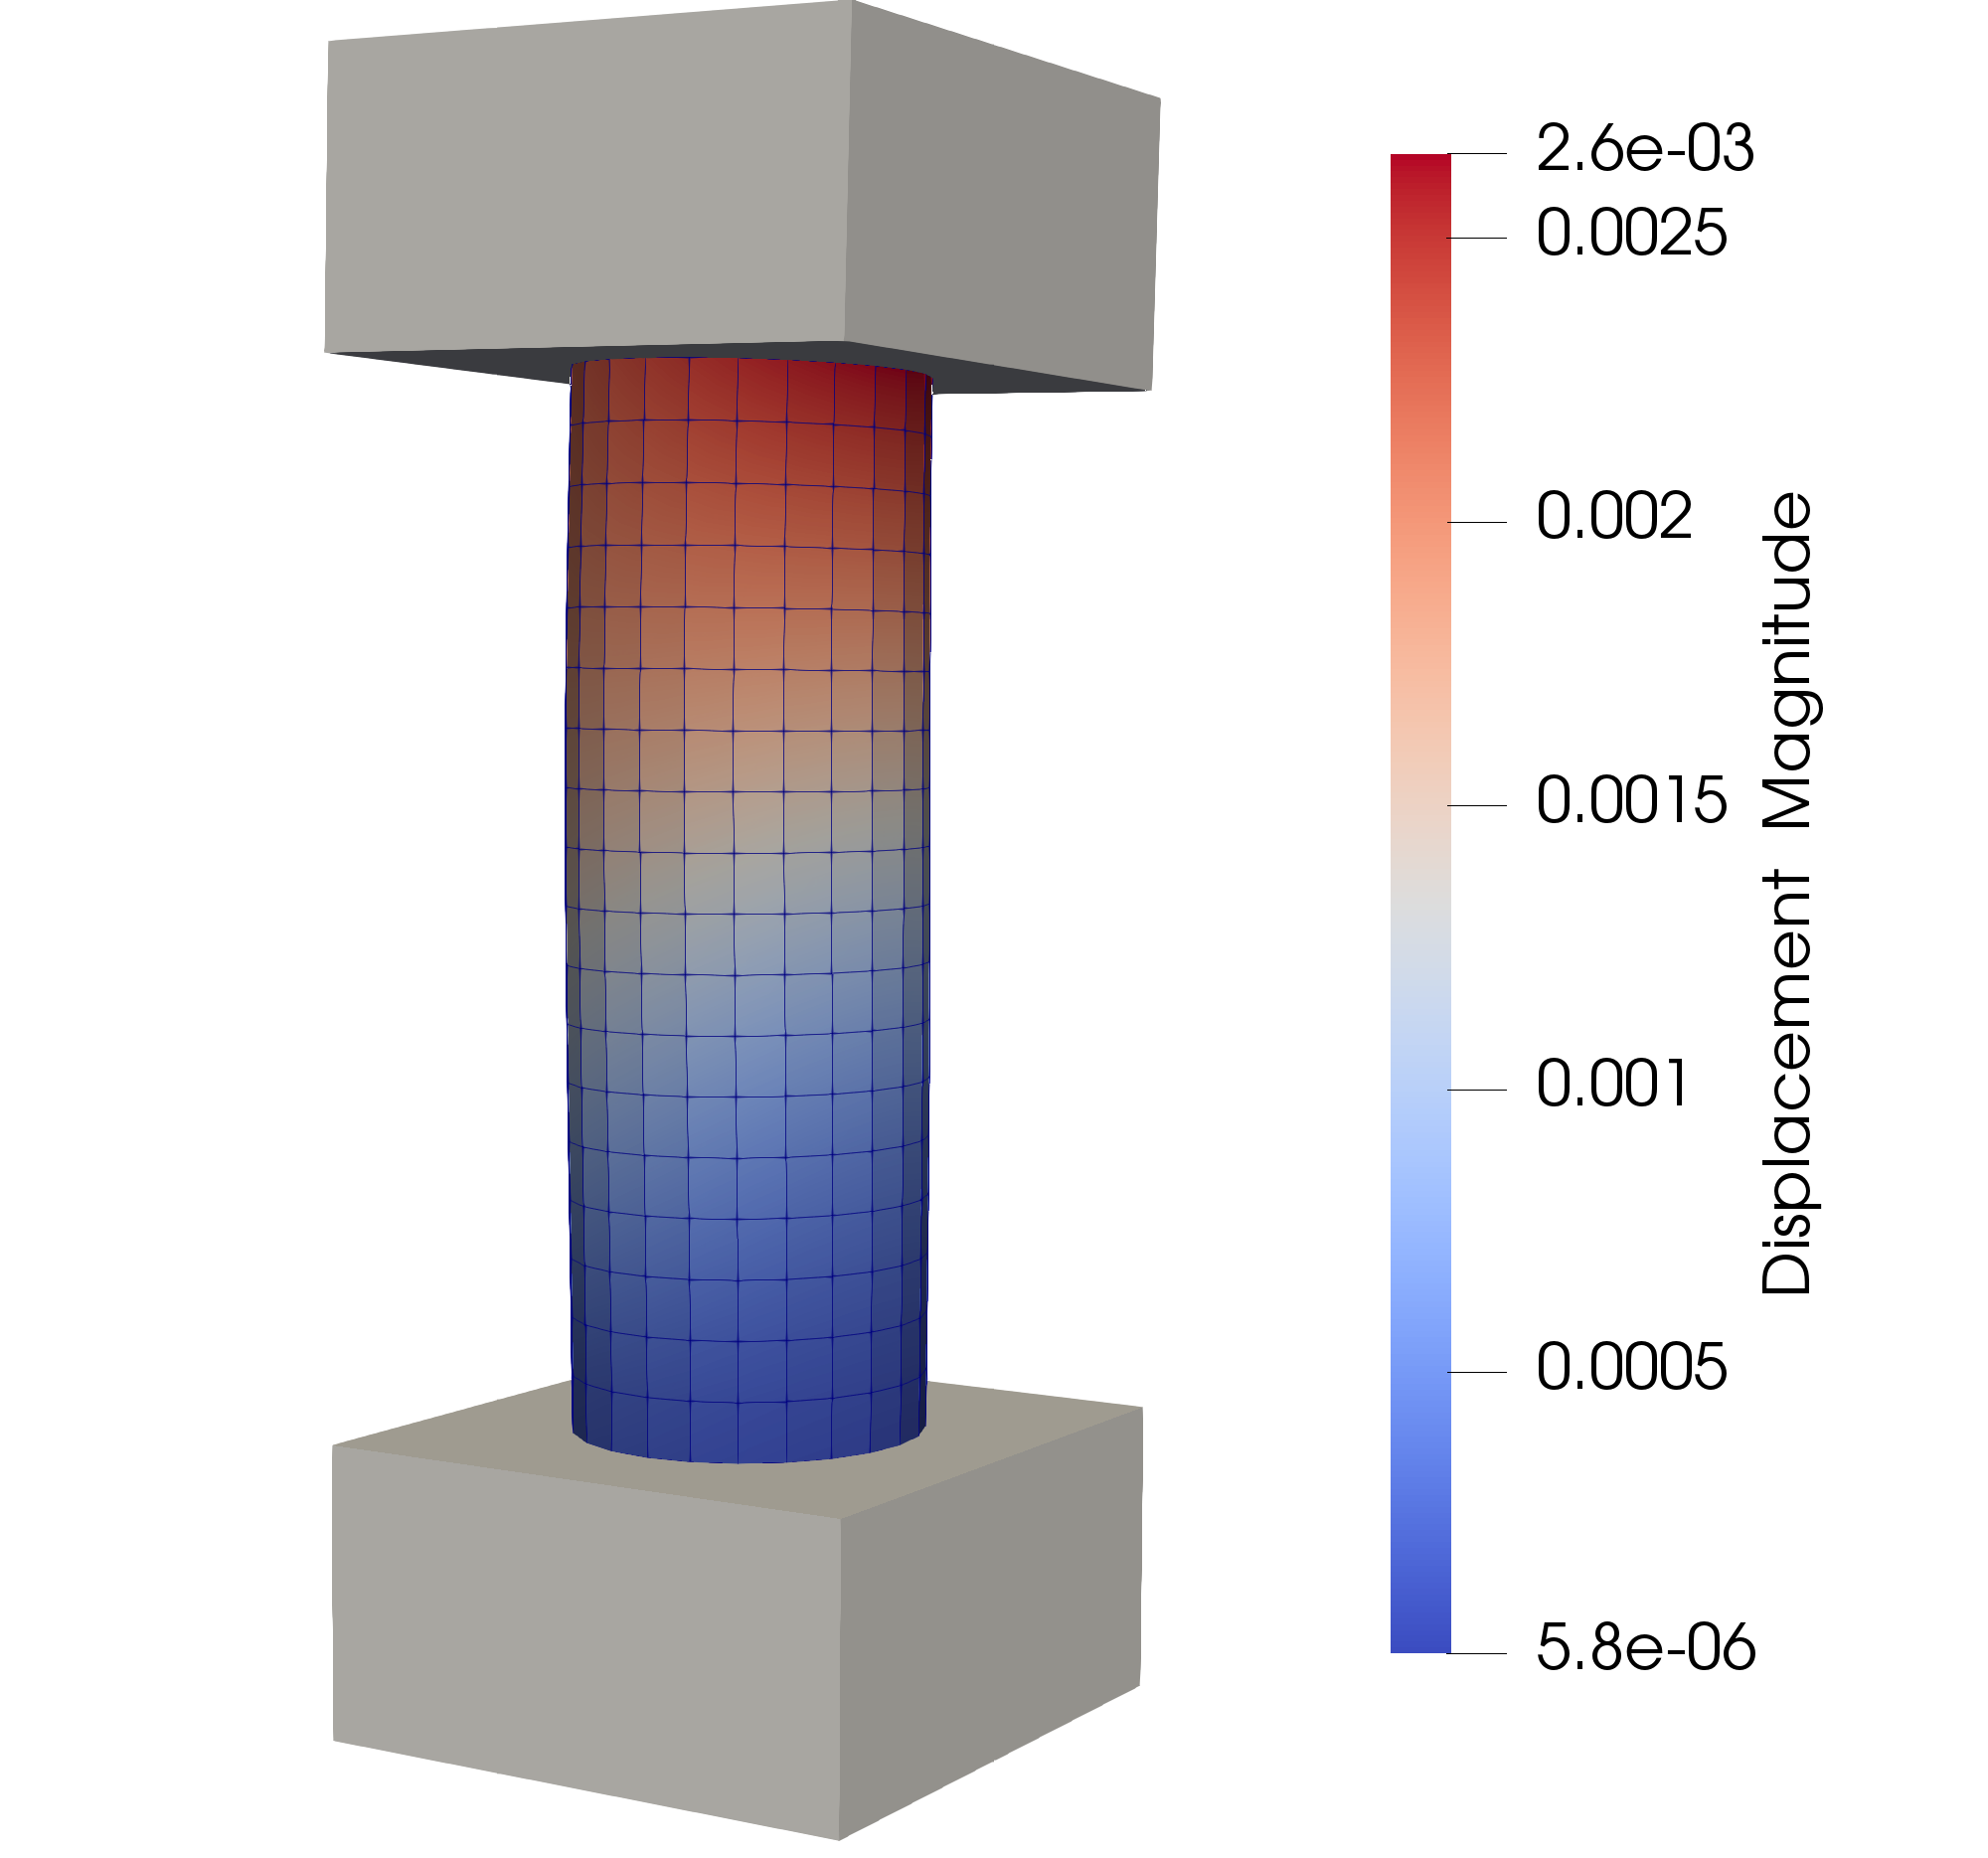
\includegraphics[width=0.6\textwidth]{obrazky/Compresion_test_3d.png}
	\caption[Compression test sample]{Compression test sample: on the surface you can see computed magnitude of displacement of the Drucker-Prager model without hardening of parameters.}\label{obr:Compresion_test}
\end{figure}

In the Fig \ref{obr:Compresion_test} you can see a slightly rotated deformation from the Z axis, which is caused the displacement of the sample from the top plate and its rotation. 

\begin{figure}[h!]
	\centering
	\includegraphics[width=1\textwidth]{obrazky/compression_test.eps}
	\caption[Compresion tests]{Compression tests compared to the real specimen result \cite{Deuch_phd_thesis}}\label{obr:Compresion_2d}
\end{figure}


The most important graph, where we can compare model accuracy to the real behavior is the Fig \ref{obr:Compresion_2d}. First line are experimental data taken from \cite{Deuch_phd_thesis}, other are results from test of the Drucker-Prager model. Red line represent Drucker-Prager model, where $M_{JP}$ is computed with Eq. (\ref{eq:f_Mjp_30}), second blue with Eq. (\ref{eq:f_Mjp_-30}) and the last, orange is computed with Eq. (\ref{eq:f_Mjp_i}). This three computations have constant cohesion $c$ and angle of friction $\varphi$. Fourth line is model with hardening of cohesion $c$, which have constant value of $20~\mathrm{MPa}$, until deviatoric plastic strain $E_d^{pl}$ increase from the value $0,05$. The second change, where cohesion become again constant with value $40~\mathrm{MPa}$, will happen when $E_d^{pl}$ reach value of $0,05$. The range between this two changes of $E_d^{pl}$ is hardening of the material. The last model is similar to the fourth with difference of cohesion parameters, which are constant from the start with value of $15~\mathrm{MPa}$ and increase to $60~\mathrm{MPa}$, when $E_d^{pl}$ reach value of $0,15$. 

In the Graph we can see that Drucker-Prager model without hardening simulate behavior with the least precision. Beginning of the computation is similar, but then real specimen started to increase deformation with higher speed. The fourth model is more precise than models without hardening, as it approaches direction of deformation increasing with the real test. But it have too much strength, which is greatly inaccurate. The last model mimics the behavior of the material most of all the simulations performed, which shows that variability of hardening/softening of the material parameters can help model to be more precise. But used approach with changing only cohesion $c$ parameter can be slightly inaccurate in high deformations of the material. This can be improved to the future with changing of angle of friction $\varphi$ and higher amount of intervals, which could more approximate real material behavior. Another solution, which can be done to the future is implementing of the Cap model to the Drucker-Prager, which is compression strength limit of the material. This has the effect to the yield of plasticity, which, when subjected to high compressive stress, turns to the axis volumetric stress. 



\begin{figure}[h!]
	\centering
	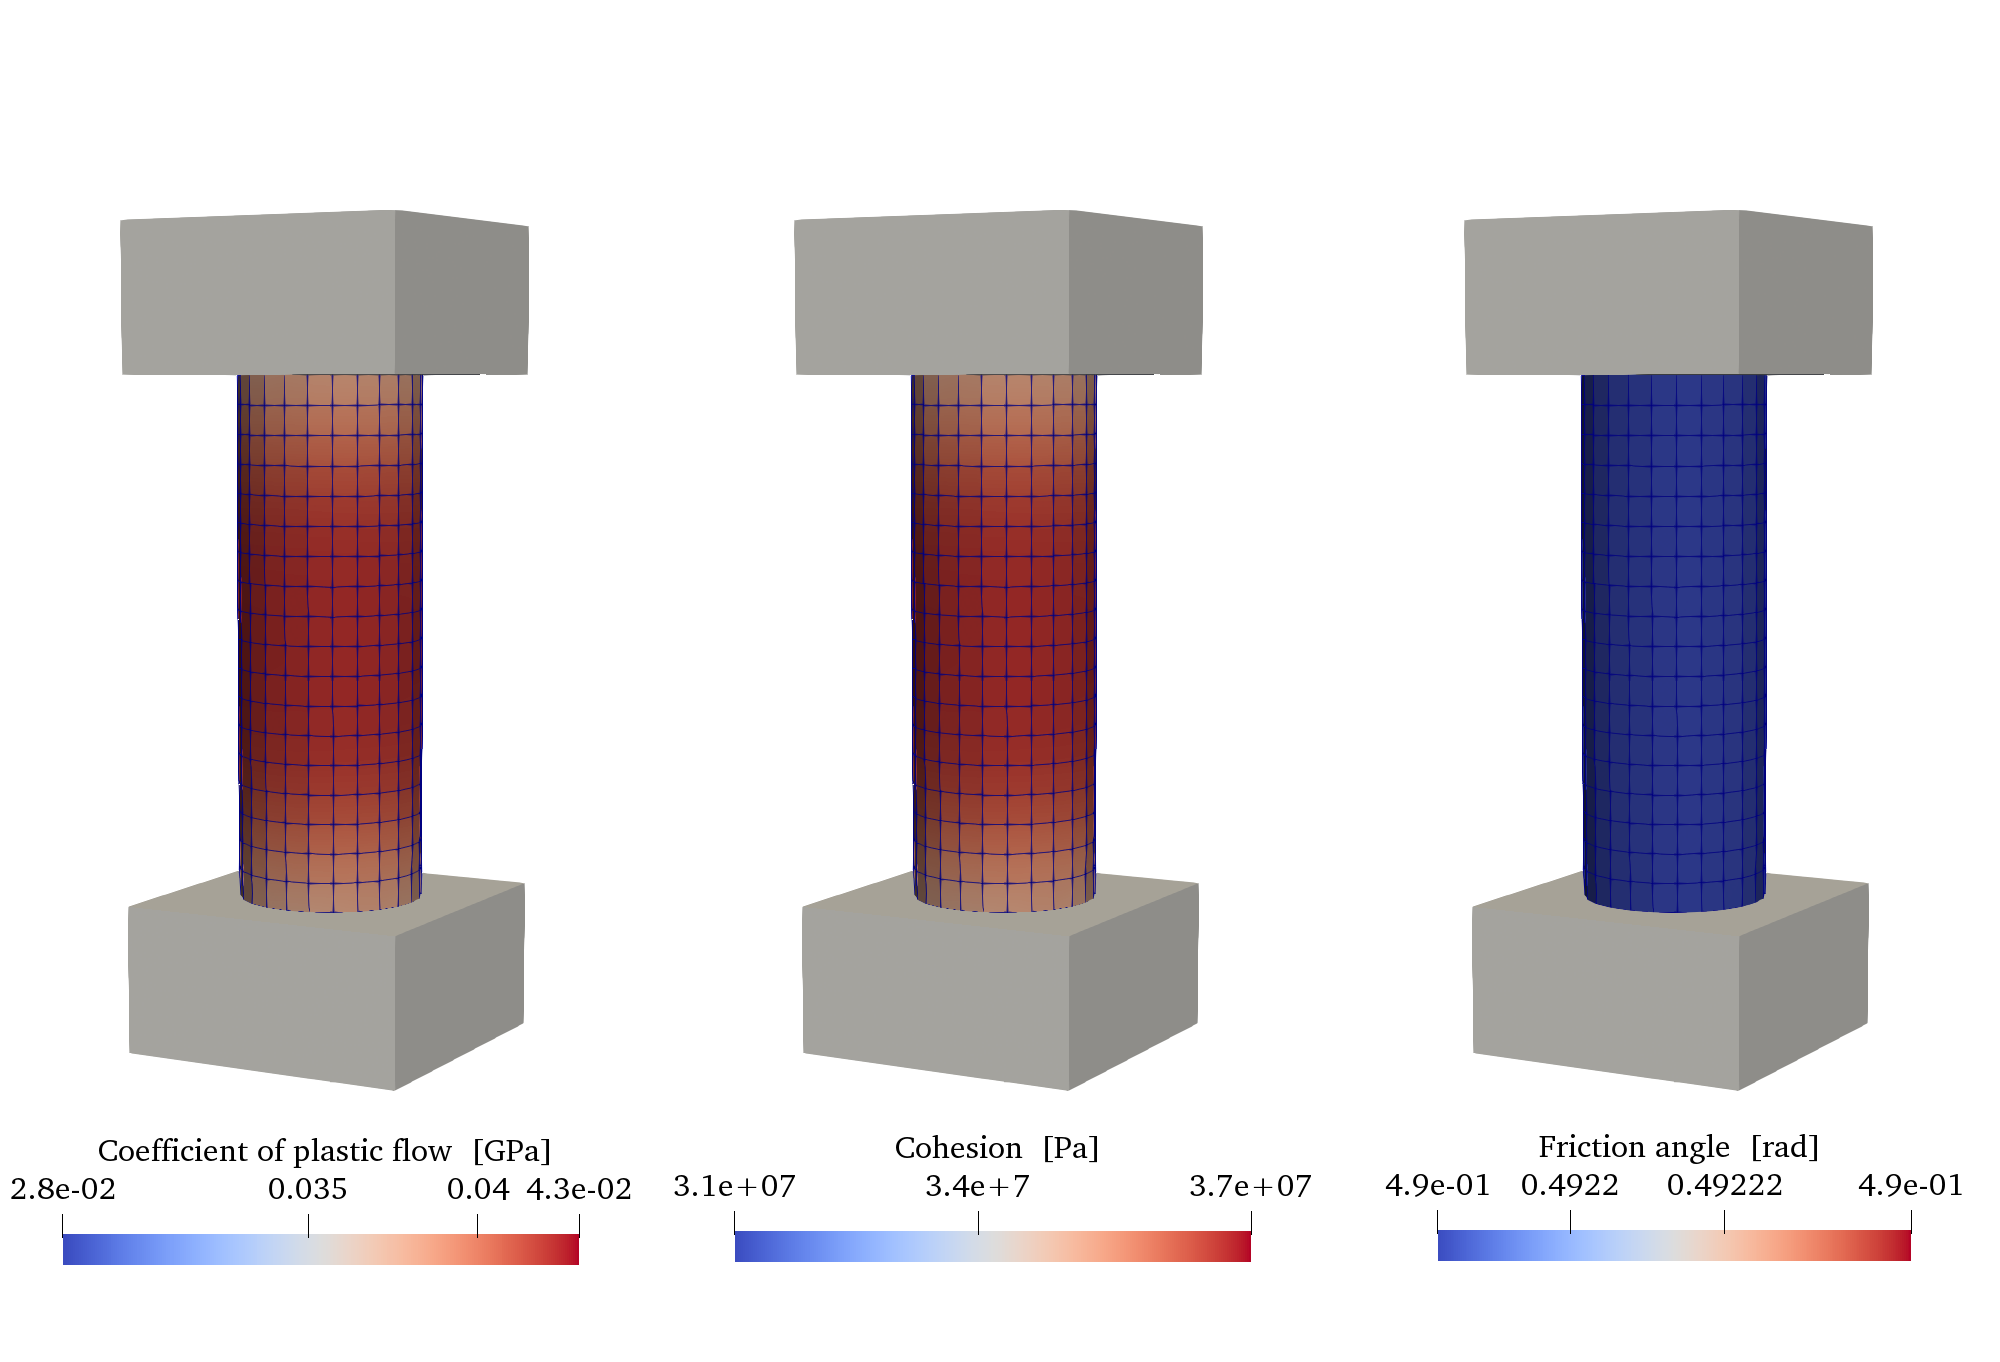
\includegraphics[width=0.6\textwidth]{obrazky/compression_zpevneni_parametry.png}
	\caption[Types of anchors]{Types of anchors ($h_{ef}$ is effective anchor length) \cite{anchors-ACI-318M}: a) cast-in-place; b) post-installed.}\label{obr:Compresion_parameters}
\end{figure}

All next Figs. of Drucker-Prager compresion test \ref{obr:Compresion_parameters}, \ref{obr:Compresion_plastic_srain} and \ref{obr:Compresion_total_strain} are from the model with hardening of cohesion $c$. In the Fig \ref{obr:Compresion_parameters} you can see that the angle of friction is constant, but cohesion is changing with increasing of deviatoric plastic strain. When we compare Figs \ref{obr:Compresion_plastic_srain} and \ref{obr:Compresion_total_strain}, we can see that distribution of the strain is similar.



\begin{figure}[h!]
	\centering
	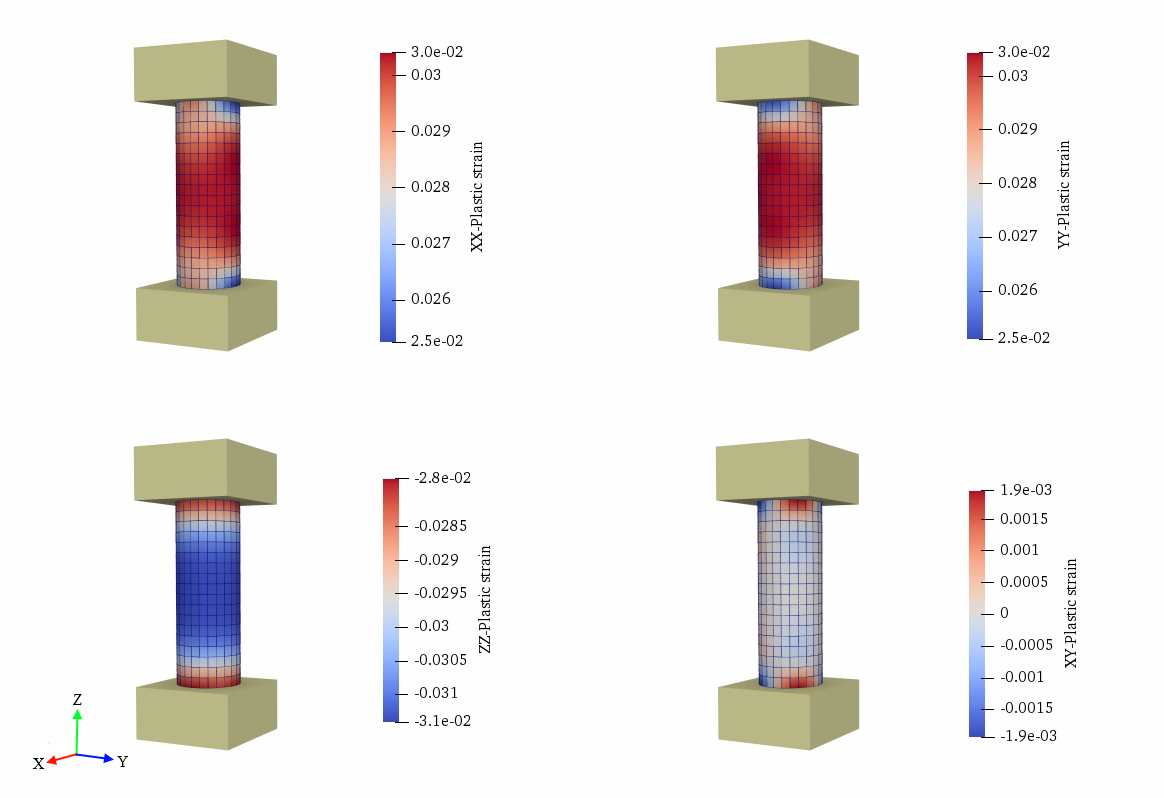
\includegraphics[width=0.7\textwidth]{obrazky/compression_zpevneni_pl_strain.png}
	\caption[Types of anchors]{Types of anchors ($h_{ef}$ is effective anchor length) \cite{anchors-ACI-318M}: a) cast-in-place; b) post-installed.}\label{obr:Compresion_plastic_srain}
\end{figure}


\begin{figure}[h!]
	\centering
	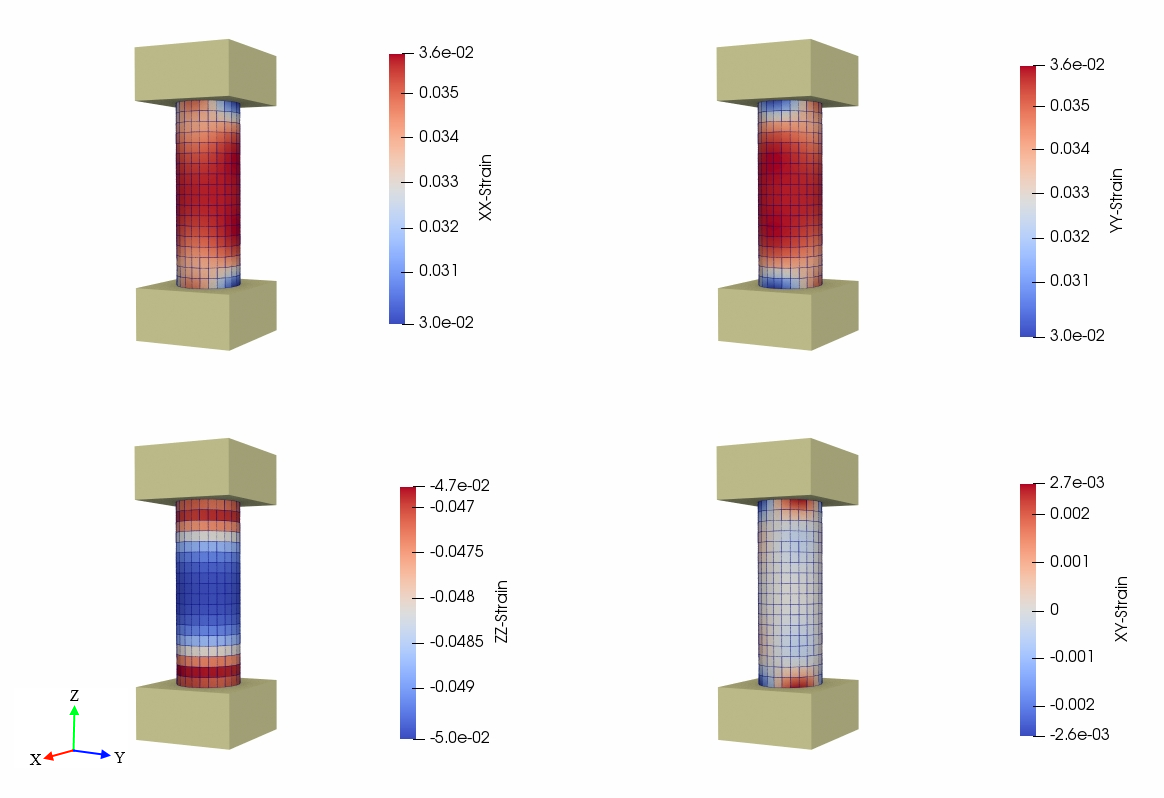
\includegraphics[width=0.9\textwidth]{obrazky/compression_zpevneni_strain.png}
	\caption[Types of anchors]{Types of anchors ($h_{ef}$ is effective anchor length) \cite{anchors-ACI-318M}: a) cast-in-place; b) post-installed.}\label{obr:Compresion_total_strain}
\end{figure}

\subsection{Results of curing model}
\indent

Curing model were already implemented into Mars FEM solver, but when we want to use it, we need to compare results of the computation with article, where was model presented \cite{heinrich2012generation}. In the Fig. \ref{obr:Curing_cube} we can see that the curing is distributed with most cured material in the center of the cube and 


\begin{figure}[h!]
	\centering
	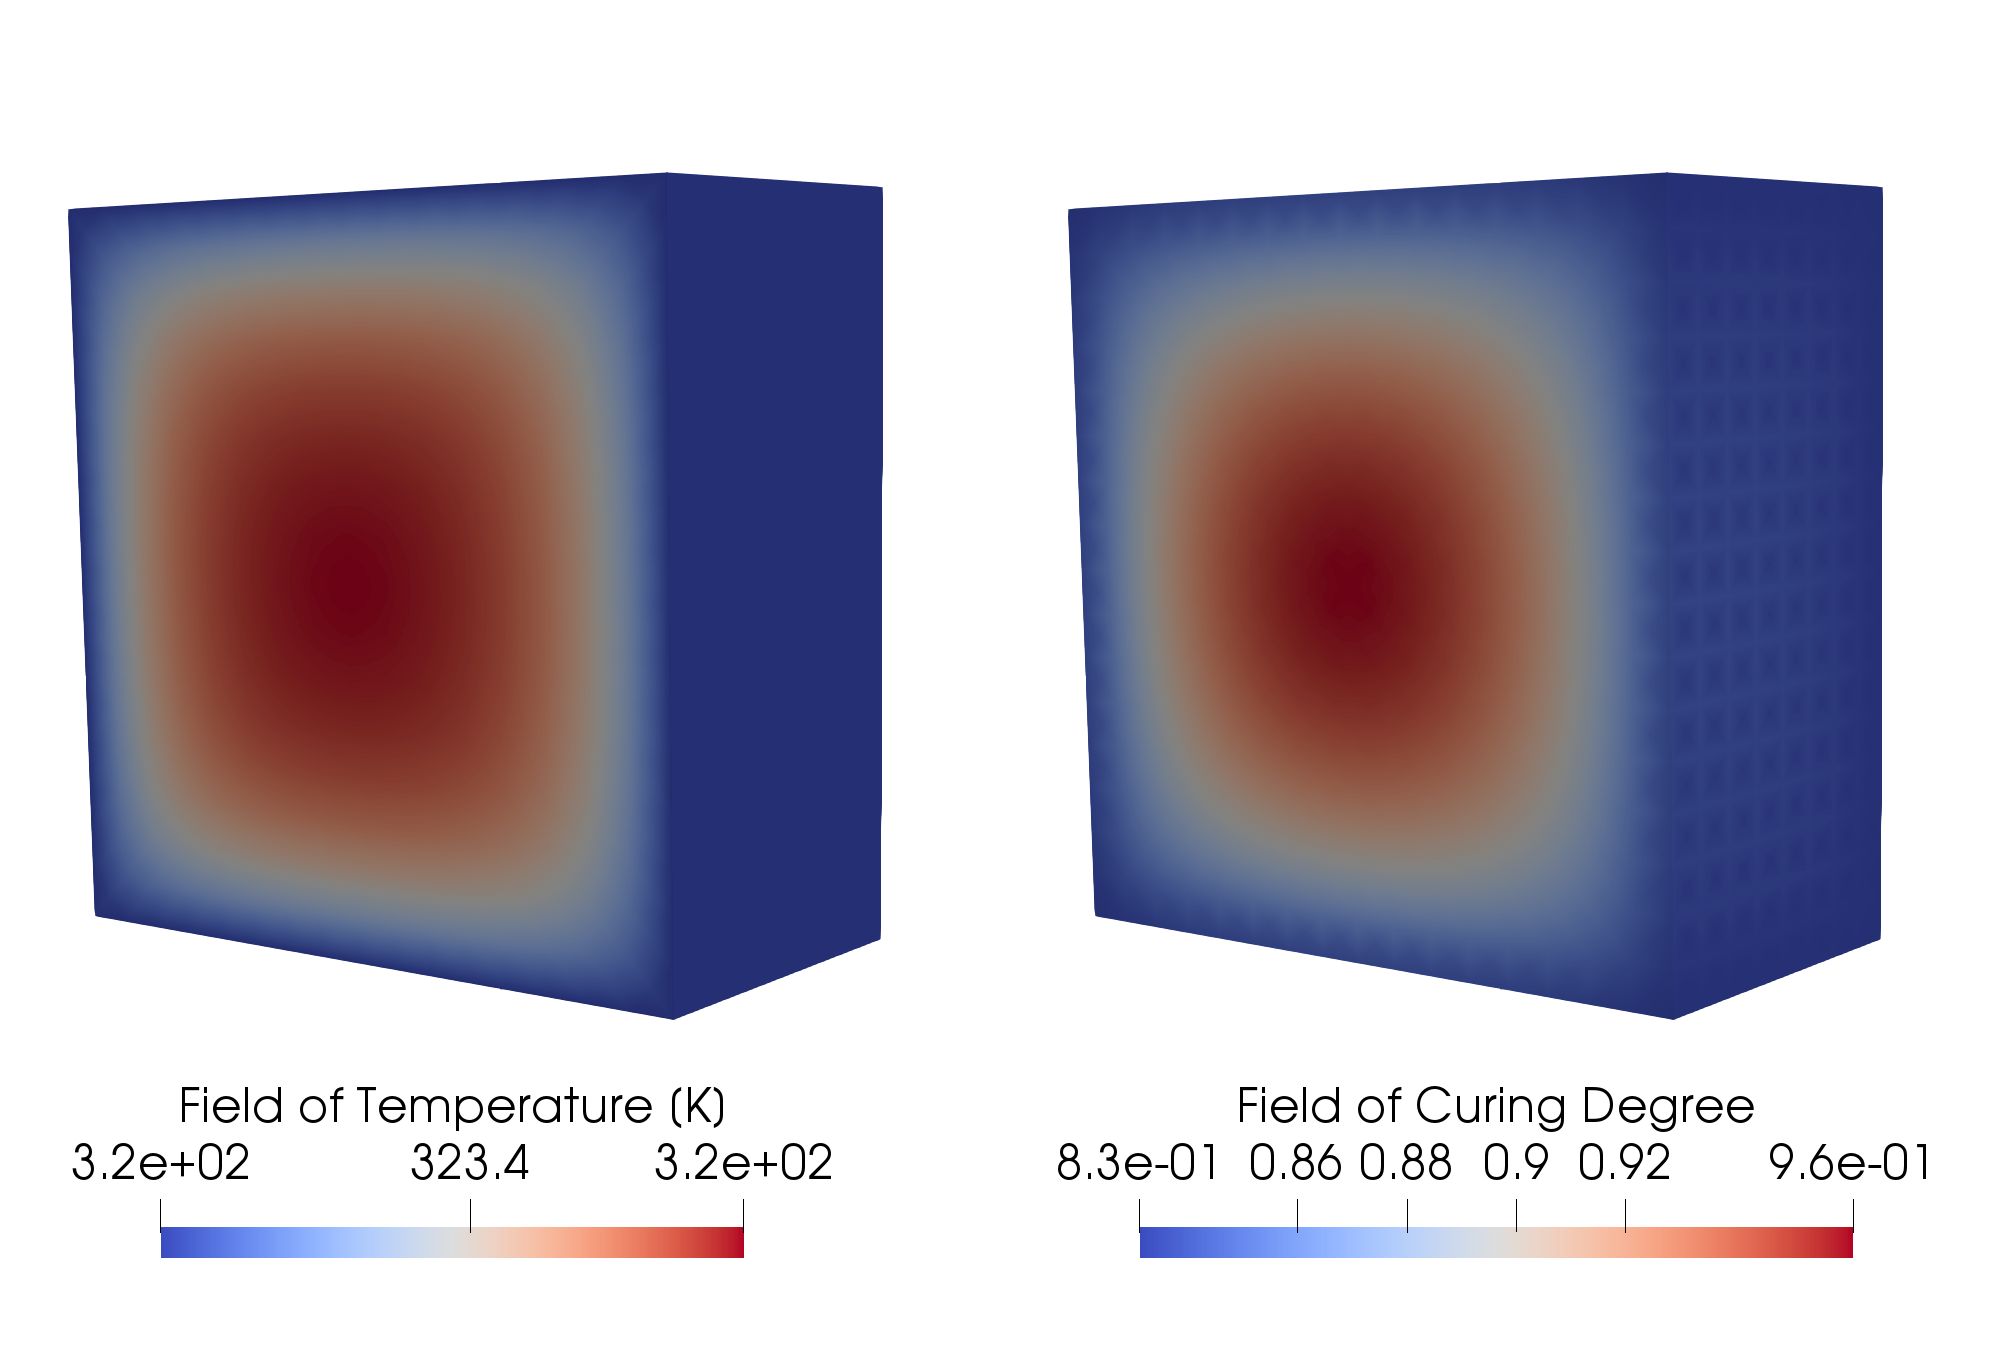
\includegraphics[width=0.9\textwidth]{obrazky/curing__and_temperature.png}
	\caption[Types of anchors]{Types of anchors ($h_{ef}$ is effective anchor length) \cite{anchors-ACI-318M}: a) cast-in-place; b) post-installed.}\label{obr:Curing_cube}
\end{figure}



\begin{figure}[h!]
	\centering
	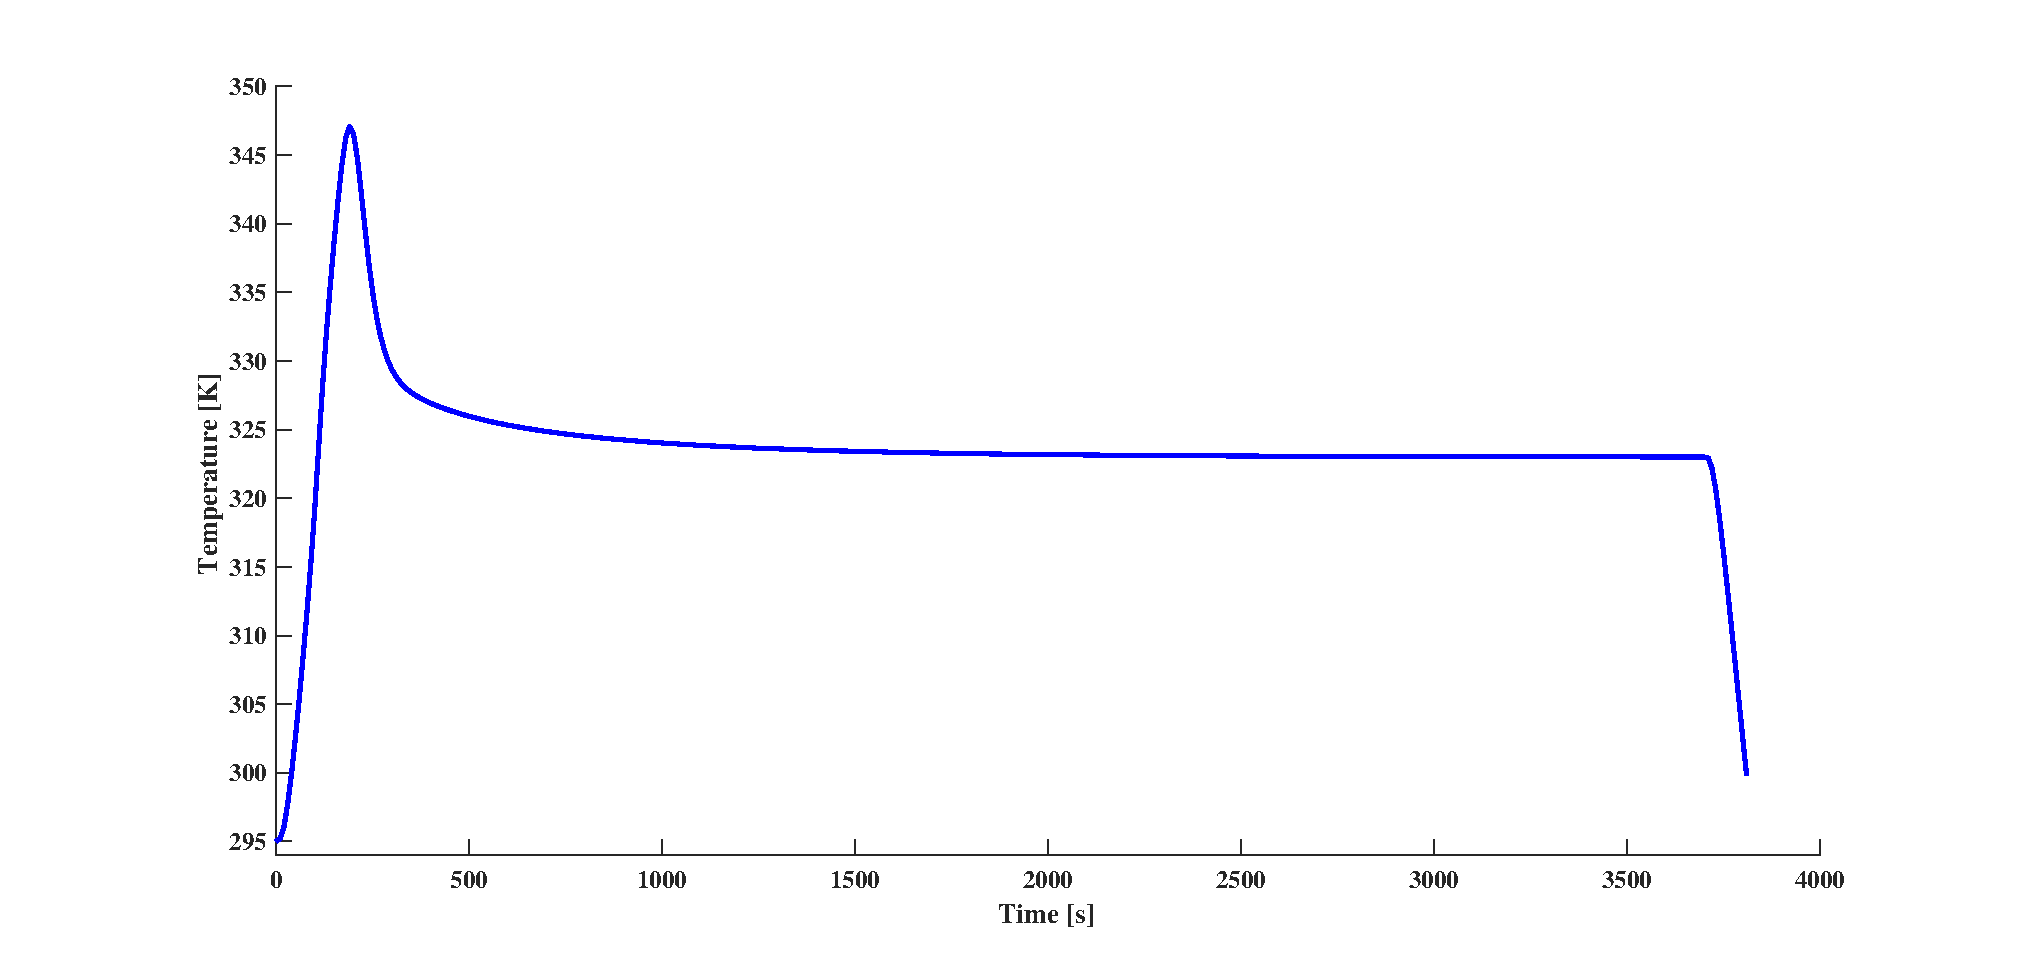
\includegraphics[width=0.9\textwidth]{obrazky/T-t.eps}
	\caption[Types of anchors]{Types of anchors ($h_{ef}$ is effective anchor length) \cite{anchors-ACI-318M}: a) cast-in-place; b) post-installed.}\label{obr:Curing_temperature}
\end{figure}

\begin{figure}[h!]
	\centering
	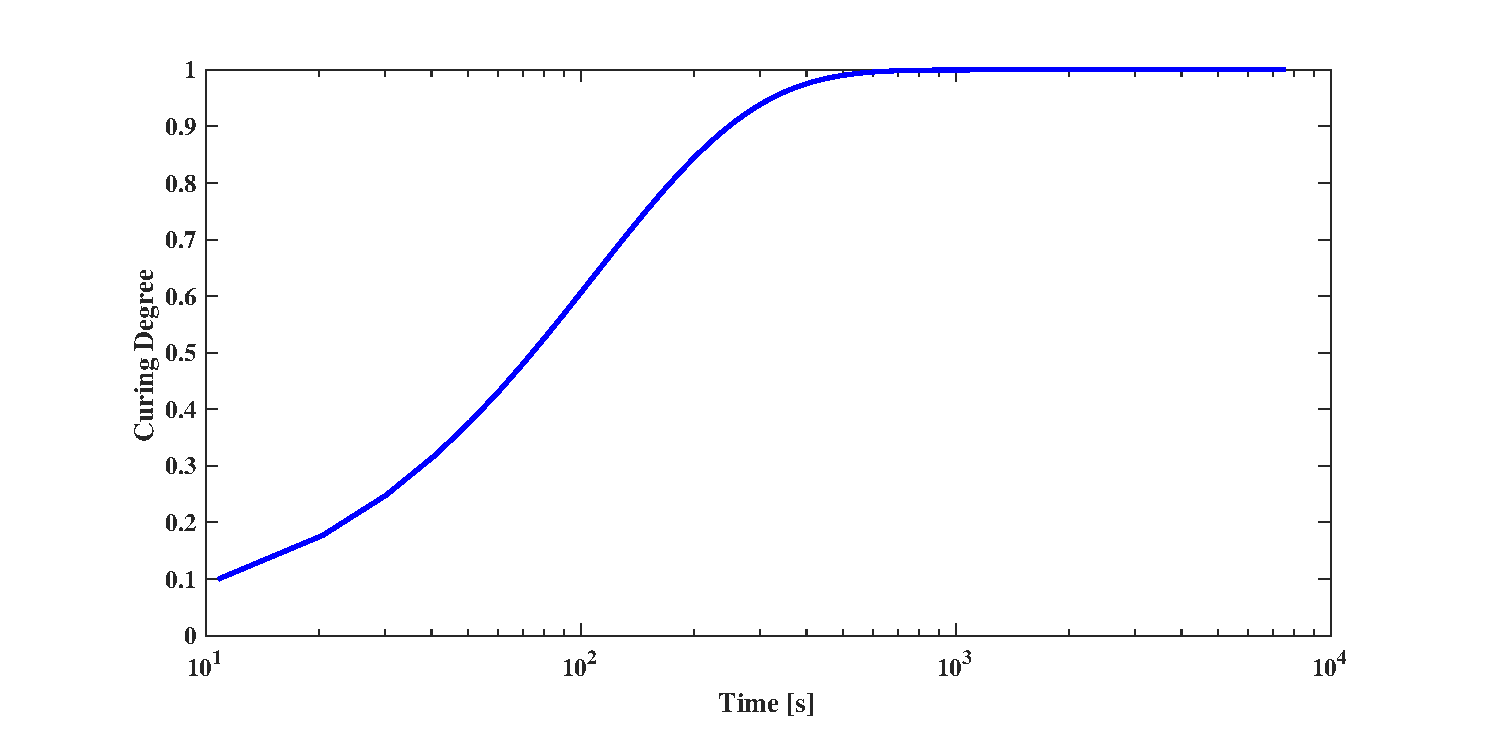
\includegraphics[width=0.9\textwidth]{obrazky/CD-t.eps}
	\caption[Types of anchors]{Types of anchors ($h_{ef}$ is effective anchor length) \cite{anchors-ACI-318M}: a) cast-in-place; b) post-installed.}\label{obr:Curing_curing}
\end{figure}
